\documentclass[10pt]{article}
\usepackage{graphicx}
\usepackage{amssymb}
\usepackage[fleqn]{amsmath}
\usepackage{nccmath}
\usepackage{cases}
\usepackage{hyperref}
\usepackage{multicol}
\usepackage{tikz}
\usepackage{pgfplots}
\usepackage{enumitem}
\pgfplotsset{compat=1.18}
\usepackage{float}
\usepackage{pdfpages}
\DeclareMathOperator*{\lcm}{lcm}

\title{\bf Math 116: Problem Set 5}
\date{2/20/2024}
\author{\bf Owen Jones}
\begin{document}
\maketitle
\begin{enumerate}[label= \arabic*.]
    \item $\phi(11413)=\phi(101)\phi(113)=100\cdot 112=11200$ $\gcd(7467,11200)=1\Rightarrow\\
    \begin{array}{c c c}
        & x & y\\
        11200 & 1 & 0\\
        7467 & 0 & 1\\
        3733 & 1 & -1\\
        1 & -2 & 3
    \end{array}\\
    \Rightarrow \phi(11413)\mid 7467\cdot 3-1\\
    \Rightarrow$ $d=3$ is our private key.\\
    Thus, $1415$ is our plaintext.
    \item $\phi(55)=40\Rightarrow 1\cdot 40+(-13)\cdot 3=1\Rightarrow d=27$\\
    \item \begin{enumerate}
        \item Every letter is encrypted to a different number modulo $n$. Knowing the public key $(e,n)$, we can create a dictionary of number letter pairs, and match each ciphertext number to its corresponding letter.
        \item $\begin{array}{c c c c c}
            A=1 & B=8192 & C=4624 & D=4028 & E=794\\
            F=2343 & G=231 & H=4461 & I=4809 & J=3556\\ 
            K=476 & L=2015 & M=513 & N=699 & O=3603
        \end{array}$\\
        HELLO is our plaintext.
    \end{enumerate}
    \item $a^1\equiv a\pmod{n}$ for all $a$. Thus, $e=1$ doesn't encrypt the plaintext. 
    $\phi(n)=p_1^{e_1-1}\phi(p_1)\ldots p_k^{e_k-1}\phi(p_k)$. 
    $\phi(p)=p-1$ is an even number for any odd prime, so $\phi(n)$ is even. 
    Thus, $e=2$ is not relatively prime to $\phi(n)$.
    \item Becuase $e$ is suitably chosen, this means $\gcd(e,\phi(p))=1$. 
    Use extended Euclidean algorithm to find integer $d$ s.t $de\equiv 1\pmod{\phi(p)}$. 
    Because $p$ is prime, $\phi(p)=p-1$. 
    The security of RSA relies on $n$ being difficult to factor. i.e $\phi(n)$ is hard to compute.
    However, primes are very easy to factor because all their factors are trivial, $1$ and $p$.
    Thus, $p$ is a poor choice to be used in an RSA encryption.
    \item ${(2^e c)}^d=2^{ed}{(m^e)}^{d}=2^{1+k\phi(n)}m^{1+k\phi(n)}\equiv 2m\pmod{n}$.
    Since $n$ is a product of two odd primes, $n$ is odd, so $2$ and $n$ are coprime. 
    Thus, we can use the extended Euclidean algorithm to find $2$'s multiplicative inverse modulo $n$.
    $2'\cdot 2m\equiv m\pmod{n}$ which gives us Nelson's original message.
    We can consider this a chosen ciphertext attack.
    \item \begin{enumerate}
        \item Eve can compute $x^{-e}$ using the extended Euclidean algorithm because $x^{-e}x^e\equiv 1\pmod{n}$.
         Let $m^c=10^{100e}\pmod{n}$. 
        She creates two lists $cx^{-e}\pmod{n}$ for $1\le x\le 10^9$ and $m^c y^e\pmod{n}$ for $1\le y\le 10^9$.
        If there is a match between the two lists, $m=xy$.
        \item Let $L$ be the length of the message $m$. 
        $m\lVert m=m(10^L+1)$.
        Let $m^c={(10^L+1)}^e\pmod{n}$. 
        She creates two lists $cx^{-e}\pmod{n}$ for $1\le x\le 10^9$ and $m^c y^e\pmod{n}$ for $1\le y\le 10^9$.
        If there is a match between the two lists, $m=xy$.
    \end{enumerate}
    \item If $e_A$ and $e_B$ are relatively prime, there exist integers $x,y$ s.t $xe_A+ye_B=1$. 
    It follows $c_A^x\cdot c_B^y\equiv m^{xe_A}m^{ye_B}\equiv m^{xe_A+ye_B}\equiv m\pmod{n}$.
    \item \begin{enumerate}
        \item If $M$ is a multiple of $p-1$ and $q-1$, there exists integers $k_1$ and $k_2$ s.t $M=k_1(p-1)$ and $M=k_2(q-1)$. 
        By Fermat's little theorem, $a^M\equiv {(a^{p-1})}^{k_1}\equiv 1\pmod{p}$, and the same idea holds for $q$.
        Because $a^M\equiv 1\pmod{p}$ and $a^M\equiv 1\pmod{q}$, the Chinese remainder theorem guarantees a unique solution $a^M\equiv x\pmod{n}$ for some $x$. 
        Because $a^M=1+kpq$ for some $k$ satisfies the system of system of congruences, $x=1$ must be the unique solution modulo $n$. 
        \item If $ed\equiv 1\pmod{M}$ then $a^{ed}\equiv a^{1}\cdot a^{kM}\equiv a^1\cdot {(a^M)}^k\equiv a\pmod{n}$
    \end{enumerate}
    \item $880525^2\cdot 2057202^2\equiv 6\pmod{2288233}$\\
    $\Rightarrow 2288233\mid(880525\cdot 2057202-648581)(880525\cdot 2057202+648581)$\\
    $\gcd(880525\cdot 2057202-648581,2288233)=1871$ is a non-trivial factor of $2288233$. The other factor is $1223$.
    \item Given $m^{12345}\equiv 1\pmod{n}$, we know $ord(m)\mid 12345$.
    We want to find $d$ st. $ed\equiv 1\pmod{ord(m)}$. 
    Since $\gcd(12345,e)=1$, pick $d\equiv e^{-1}\pmod{12345}$ using the extended Euclidean algorithm.
    Thus, $c^d\equiv m^{ed}\equiv m^{12345k+1}\equiv {(m^{12345})}^k\cdot m\equiv m\pmod{n}$.
    \item 
    \begin{enumerate}
            \item \begin{align*}
                m'\equiv m_1\equiv c^{d_1}\equiv m^{ed_1}\equiv m^{1+k_1(p-1)}\equiv m\pmod{p}\\
                m'\equiv m_2\equiv c^{d_2}\equiv m^{ed_2}\equiv m^{1+k_2(q-1)}\equiv m\pmod{q}
            \end{align*}\\
            for integers $k_1,k_2$.
            By the uniquess of CRT, $m'=m+kpq$ for some integer $k$ satisfies the system of congruences. Thus, $m'\equiv m\pmod{n}$
            \item $m'=m_1qy+m_2px\pmod{n}$.
    \end{enumerate}
    \item $60103201518091407091908011804$
    \item $n=835338435834994481423891073871\times 897930023819537415148640533529$
    \item $2,3$, and $5$ all fail to show $n$ is composite $7^{n-1}\equiv 10334100\pmod{n}$
    \item \begin{enumerate}
        \item For bases $b=2,3$ $b^{n-1}\equiv 1\pmod{n}$, so we conclude $n$ is probably prime.
        \item Base $b=3$ proves $n$ is composite giving non-trivial factor $520801$. Other factor is $3361$.
    \end{enumerate}
\end{enumerate}
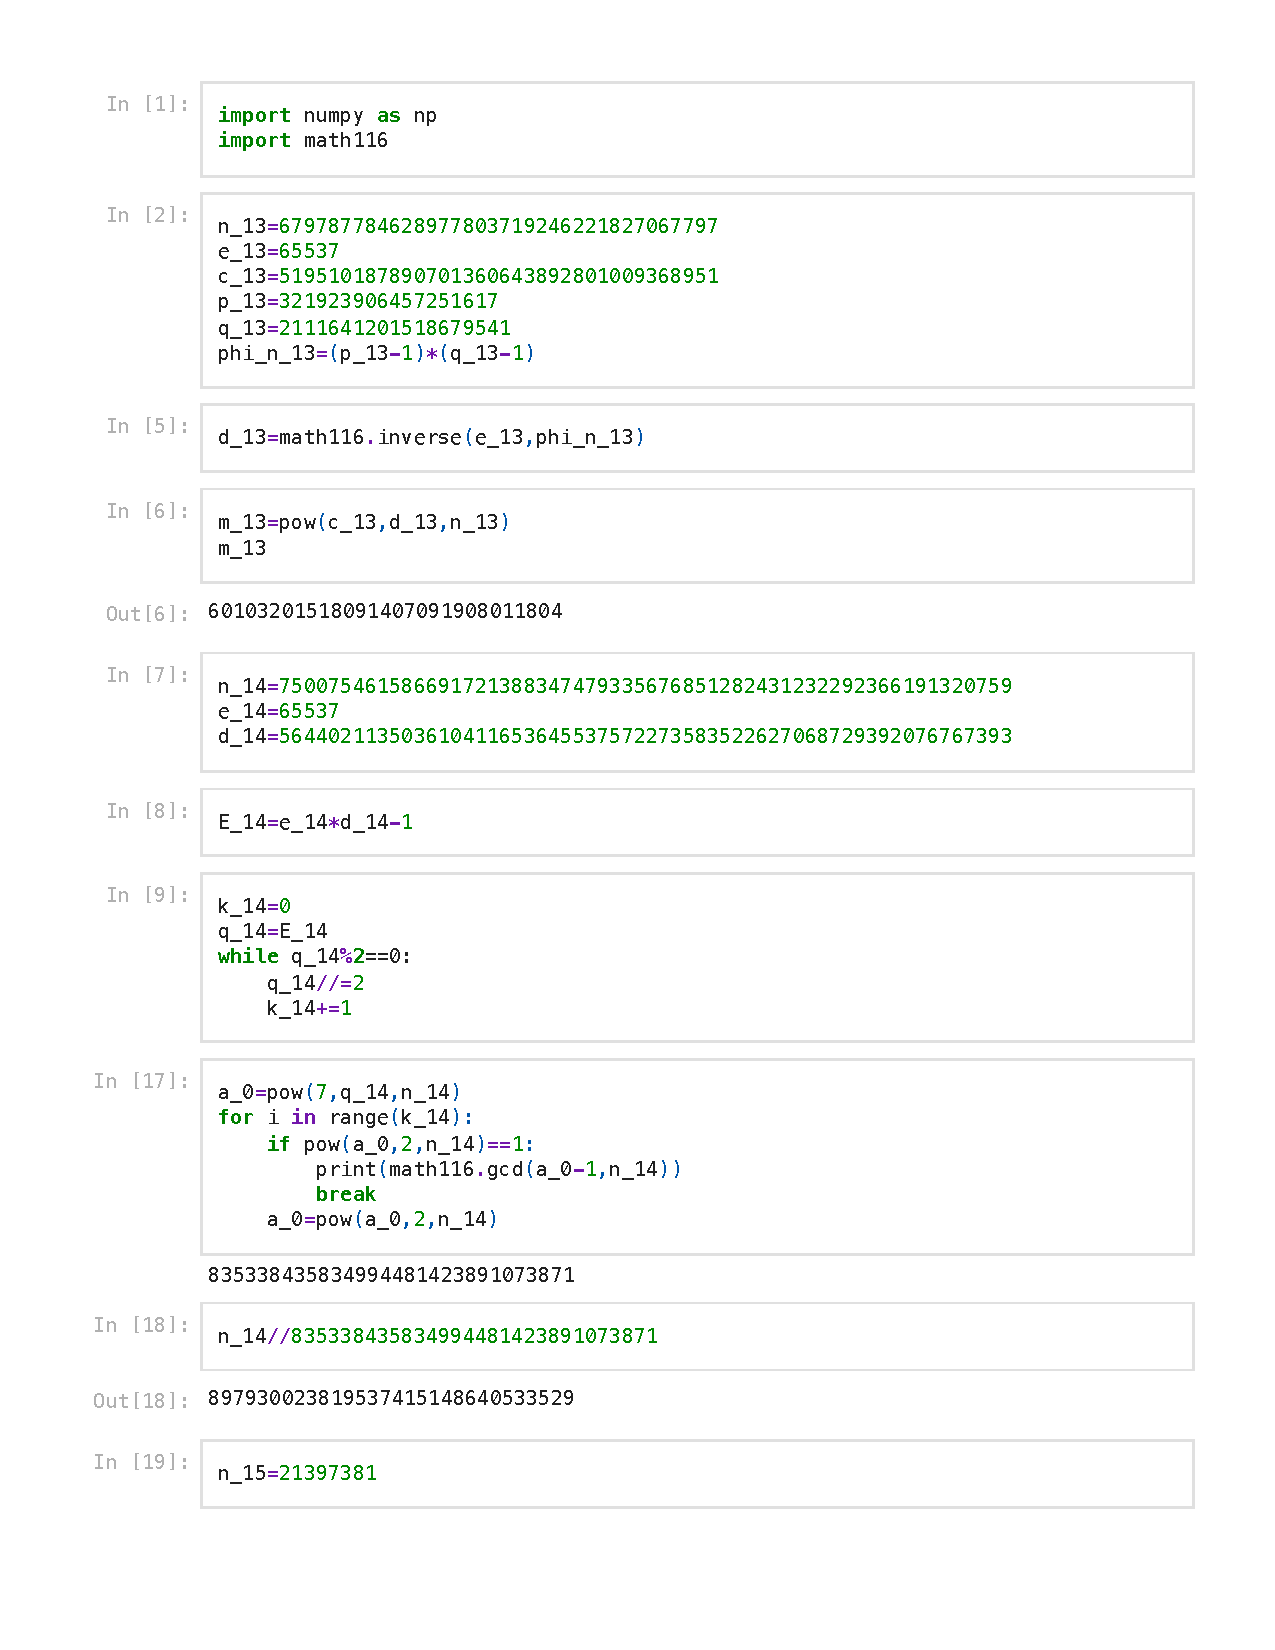
\includepdf[pages=-]{homework_5_116.pdf}
\end{document}